\section{Einleitung}
Die wissenschaftliche Forschung wurde als wichtiger Einflussfaktor für die Entstehung neuer Technologien und Technologietrends in bedeutenden Studien nachgewiesen.\footnote{\citeNP<Vgl.>[S.~187.]{Nelson1986}}\footnote{\citeNP<Vgl.>[S.~11.]{Mansfield1991}}\footnote{\citeNP<Vgl.>[S.~599.]{Tegarden2012}}
Nach \shortciteauthor{Jaffe1989} wird diese Erkenntnis bereits durch die geographische Nähe von Zentren der Spitzentechnologie wie das \glqq Silicon Valley\grqq~oder die "`Massachusetts Route 128"' zu führenden Universitäten gestützt.\footnote{\citeNP<Vgl.>[S.~967f.]{Jaffe1989}} Einer Studie von \shortciteauthor{Mansfield1991} zufolge wären etwa 11~\% aller Produkte einer Auswahl aus sieben Fertigungsindustrien im Betrachtungszeitraum gar nicht oder nur mit erheblicher Zeitverzögerung entwickelt worden, wäre dem nicht eine entsprechende wissenschaftliche Forschung vorausgegangen.\footnote{\citeNP<Vgl.>[S.~2.]{Mansfield1991}}

Dennoch liegt die maßgebliche Entscheidung über den Einsatz und die Weiterentwicklung neuer Technologien vorwiegend in Händen von Unternehmern, Managern und sonstigen Entscheidungsträgern der praktizierenden Wirtschaft. Die wiederum richten ihre Entscheidungen unter Berücksichtigung einer Vielzahl von Faktoren an den Markt aus, um den Unternehmenserfolg zu steigern.\footnote{\citeNP<Vgl.>[S.~1652f.]{Gruber2008}} Dabei greifen sie auch auf Informationsquellen von spezialisierten Unternehmen zurück, die mit Hilfe proprietärer Methoden Prognosen für Technologietrends in eigenen Publikationen herausgeben. Einer der einflussreichsten und bekanntesten Vertreter dessen ist der "`Gartner Hype Cycle"', den große Unternehmen bei strategischen Entscheidungen bezüglich neuer Technologien beratend hinzuziehen.\footnote{\citeNP<Vgl.>[S.~254.]{Steinert2010}}

Nach \shortciteauthor{Beyer1992} ist der Einfluss auf Technologietrends durch Wirtschaftsmedien höher als durch wissenschaftliche Artikel, da sie von Managern aufgrund des gewohnten Fachjargons sowie der Praxisrelevanz bevorzugt gelesen werden.\footnote{\citeNP<Vgl.>[S.~472.]{Beyer1992}} \shortciteauthor{Barley1988} fanden sogar heraus, dass sich gängige Begriffe der Wirtschaft in wissenschaftlicher Literatur verzögert manifestieren, folglich der Einfluss unidirektional von Unternehmern in Richtung Akademiker stattfindet.\footnote{\citeNP<Vgl.>[S.~52.]{Barley1988}} Nach \shortciteauthor{Spell1999} hängt das allerdings eher damit zusammen, dass wissenschaftliche Artikel einem \glqq Peer-Review\grqq~unterzogen werden, welcher Monate bis Jahre in Anspruch nehmen kann, bis sie in Fachartikeln erscheinen, als dass wissenschaftliche Forschungsschwerpunkte stets aus Wirtschaftsjournalen gespeist würden.\footnote{\citeNP<Vgl.>[S.~345.]{Spell1999}}

\subsection{Problemstellung}
Somit findet eine gegenseitige Einflussnahme hinsichtlich der Prognose von Technologietrends zwischen Entscheidungsträgern der Wirtschaft und akademischen Forschern zweifelsohne statt. Gleichzeitig ist aufgrund teils unterschiedlicher Interessen beider Parteien eine Diskrepanz bei der Schwerpunktsetzung evident. 

Technologiethemen insbesondere in Informationstechnologien sind ständiger Ver\-änderung unterworfen\footnote{\citeNP<Vgl.>[S.~107f.]{Chang2009}}, wodurch eine permanente Auseinandersetzung mit Trend\-themen für beide Seiten unumgänglich ist. Obwohl das "`Gartner Hype Cycle"' bei der Lösung dieser Herausforderung hohe Anerkennung in der Praxis genießt, bleibt es in der akademischen Forschung weitestgehend unberücksichtigt.\footnote{\citeNP<Vgl.>[S.~241.]{OLeary2008}}\footnote{\citeNP<Vgl.>[S.~12.]{Jarvenpaa2008}}

In einer aktuellen Studie über das Thema \glqq Enterprise Architecture\grqq~wurden Anhaltspunkte für Diskrepanzen zwischen Trendthemen des \glqq Gartner Hype Cycle\grqq~und der akademischen Forschung festgestellt, die weiterer Untersuchung bedürfen.\footnote{\citeNP<Vgl.>[S.~82.]{Gampfer2018}} Darauf aufbauend geht es um die Frage, ob und in welchem Ausmaß sich Technologietrends in der wirtschaftlichen Praxis von denen der wissenschaftlichen Forschung unterscheiden.

\subsection{Zielsetzung}
Das vorrangige Ziel der Arbeit ist es, über einen definierten Zeitraum Technologiethemen mit der höchsten medialen Präsenz in der Wirtschaft zu erfassen und die Verteilung dieser Themen in wissenschaftlichen Fachartikeln im Verhältnis gegenüberzustellen.

Dazu wird eine Datenbasis der Trendthemen aus dem "`Gartner Hype Cycle for Emerging Technologies"' für einen bestimmten Betrachtungszeitraum erhoben, um schließlich mit Hilfe quantitativer Methoden eine Gegenüberstellung durchzuführen.

Als Ergebnis der Analyse wird die Erkenntnis angestrebt, mögliche Diskrepanzen beim Verständnis für vielversprechende Trends festzustellen.

\subsection{Leitfragen}
Die einleitend genannte Feststellung, dass sich akademische Forschungsschwerpunkte im Bereich von neuen Technologien mit zeitlicher Verzögerung zur wirtschaftlichen Praxis etablieren, ist zum Ende des letzten Jahrhunderts gemacht worden. Der "`Gartner Hype Cycle"' ist etwa zur gleichen Zeit erstmalig im Jahre 1995 erschienen\footnote{\citeNP<Vgl.>[S.~241.]{OLeary2008}} und findet folglich in diesen Artikeln keine Berücksichtigung.

Um die Aktualität dieser Erkenntnis zu eruieren, werden hieraus folgende Leitfragen abgeleitet:

\begin{description}
	\item[L1:] Wie ist das Verhältnis zwischen Technologien im Abschnitt "`Peak of Inflated Expectations"' und der Anzahl an wissenschaftlichen Publikationen im vergleichbaren Zeitraum?
\end{description}

\begin{description}
	\item[L2:] Ist eine erstmalig erschienene Technologie des "`Gartner Hype Cycle"' im Ab\-schnitt "`Peak of Inflated Expectations"' in wissen\-schaftlichen Ver\-öf\-fent\-lichungen als Trend wahrzunehmen?
\end{description}

\begin{description}
	\item[L3:] Wenn eine Technologie in einer späteren Ausgabe des "`Hype Cycle"' herausfällt, steigt die Anzahl wissenschaftlicher Artikel um eine gewisse Zeit weiter, bis sie stagniert bzw. abnimmt?
\end{description}

Durch die retrospektive Analyse vergangener Trendthemen können mit heutiger Betrachtung möglicherweise weitere Leitfragen hinsichtlich der Ursachen für Abweichungen aufgestellt werden, die als Grundlage für die weitere Forschung dienen können.

\subsection{Methodik}\label{sec:method}
Wegen der eingangs erwähnten Relevanz wird der "`Gartner Hype Cycle for Emerging Technologies"' als Stellvertreter für die wirtschaftliche Praxis bei der Bestimmung kommender Trendthemen angenommen. Dabei handelt es sich um die graphische Darstellung des üblicherweise zu beobachtenden Reifeprozesses einer neuen Technologie.

In Abbildung \ref{fig:ghc_raw} ist der Rohaufbau einer solchen Graphik mit unter anderem dem Kurvenverlauf sowie den fünf Stufen bis zur Produktivität zu sehen. Der Abschnitt "`Peak of Inflated Expectations"' zeigt die Phase mit den größten, meist überzogenen Erwartungen an die Technologie, in der auch die Medienpräsenz am höchsten ist.\footnote{\citeNP<Vgl.>[S.~3f.]{Fenn2017}} Deshalb werden die dort aufgeführten Technologien einer aktuellen Ausgabe als Grundlage für den Trendvergleich verwendet.

\begin{figure}
	\centering
	\caption{Struktur des \glqq Gartner Hype Cycle\grqq}
	\includegraphics[clip,width=\linewidth,page=4,trim=1.8cm 12.8cm 2.5cm 3.8cm]{pdf/ghc_raw}
	\caption*{\protect\fullciteNP<Quelle:>[S.~4]{Fenn2017}}
	\label{fig:ghc_raw}
\end{figure}

Demgegenüber manifestieren sich Ergebnisse akademischer Forschung vorwiegend in wissenschaftlichen Fachartikeln sowie Konferenzbeiträgen. Diese werden nach sog. \glqq Peer-Reviews\grqq \footnote{Prüfung durch Fachgenossen} in entsprechenden Fachzeitschriften veröffentlicht.\footnote{\citeNP<Vgl.>[S.~381.]{Bucchi1996}} Spezielle Literaturdatenbanken mit einer Web-Schnittstelle bieten Möglichkeiten zur Suche und Anzeige solcher Artikel an. Für die Suche der aus dem \glqq Gartner Hype Cycle\grqq~ermittelten Technologien kommt eine Auswahl dieser Datenbanken zum Einsatz.

Die Suchbegriffe werden gegebenenfalls erweitert oder taxonomisch eingegrenzt, falls ihre Verwendung in der wissenschaftlichen Literatur signifikant abweicht und dies somit erfordert.